\documentclass[10pt,letterpaper]{article}
\usepackage[utf8]{inputenc}
\usepackage{amssymb, amsmath}
\usepackage{graphicx}
\usepackage{fancyhdr}
\usepackage{multicol}
\usepackage{multirow}
\usepackage{float}
\usepackage{wrapfig}
\usepackage{graphicx}

\usepackage{hyperref}
\renewcommand{\refname}{}
\hypersetup{
    colorlinks=true,
    linkcolor=red,
    filecolor=magenta,      
    urlcolor=blue,
    citecolor=blue,
}


\graphicspath{ {img1/} }


\usepackage[letterpaper,top=2cm,bottom=2cm,left=3cm,right=3cm,marginparwidth=1.75cm]{geometry}





\fancyhf{}
\lhead[\leftmark]{}
\rhead[]{César Ornelas}
\lfoot[\thepage]{}
\rfoot[]{\thepage}



\begin{document}

\begin{title}

\begin{wrapfigure}{r} %this figure will be at the right
    \centering
    
\includegraphics[width=4cm]{img/logos.png}
\end{wrapfigure}

Octubre 2024
\begin{center}
    \vspace{1cm}
    \hspace{1cm}
    \Large
    \textbf{Pruebas de peso para el Principio de Arquímedes} \\

    \vspace{0.5cm}

    \normalsize
    López Gónzalez A. , Hernández Gómez A. \\ Villanueva Sanluis A. , Ornelas Arias C.
    
    \vspace{0.3cm}

\end{center}
    

    
    
\end{title}

    \hline
	\section*{Resumen}

    Se demostró experimentalmente el Principio de Arquímedes. El experimento que se llevó a cabo para esto consistió en colocar un vaso de precipitado con agua sobre una báscula, y sumergir una pelota colgada de una cuerda a un dinamómetro, para registrar el peso antes y después de sumergirla. A partir de los datos obtenidos se concluyó que en efecto se cumple que $\Vec{F} = - mg \hat{y} + \rho g V \hat{y} + \Vec{F_{ext}}$.

    \vspace{1cm}

    \hline
	
    \section{Introducción}

    \hline
    
    \begin{multicols}{2}

    \subsection{Marco Teórico}

    El principio de Arquímedes lo podemos estipular de la siguiente forma \cite{hamb}:

    \begin{quote}
        Un objeto inmerso en un fluido es sostenido por una fuerza igual al peso del fluido que
        desplaza.
    \end{quote}

    Consideremos el ejemplo ilustrado en la figura \ref{ejem}, en el cual una pelota se sumerge en un liquido, donde la parte inmersa tiene un volumen $V$. Dicho fluido va a ejercer una fuerza (llamada boyante) contraria en dirección al peso del objeto mismo, y respecto a la magnitud, esta será igual al peso del agua que ocuparía el volumen $V$.
    
    Si conocemos la densidad $\rho$ de este, la magnitud de la fuerza boyante sera simplemente:
    \begin{equation}
        F_b = \rho g V
    \end{equation}

    \begin{figure}[H]
        \centering
        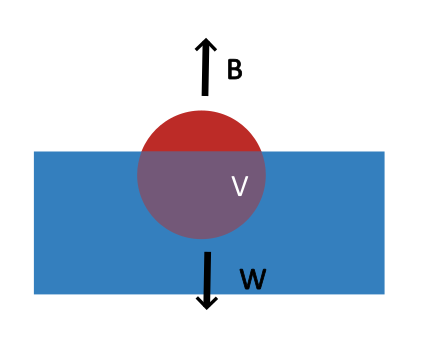
\includegraphics[width = 4.5cm]{img/img1.png}
        \caption{\label{ejem} Fuerza boyante}
    \end{figure}

    Es esta misma propiedad la que brinda flotabilidad a distintos objetos cuando se sumergen en algún fluido, como pasa con las boyas de mar o con los mismos globos dentro del aire. En la vida real podemos encontrar este fenómeno en los hielos de una bebida, donde la razón por la que flotan es debido a esta fuerza de flotación, donde la parte que queda sumergida desplaza una cantidad de agua cuyo peso es igual al del hielo, haciendo que las fuerzas se equilibren. Ahora bien, el que un objeto flote o se hunda depende justamente de la densidad tanto del objeto como del medio. Si la del primero resulta ser mayor, el peso va a ser mayor a la fuerza boyante, y se hundirá. Si por el contrario, la densidad del fluido es mayor, el objeto flota. Esto puede parecer no cierto cuando vemos, por ejemplo, barcos de acero flotando, pero hay que considerar que la forma en la que estos se moldean permiten aumentar el volumen desplazado como se muestra en la figura \ref{flot}

    \begin{figure}[H]
        \centering
        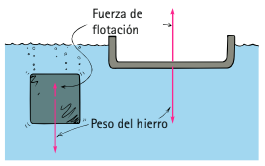
\includegraphics[width = 5cm]{img/img2.png}
        \caption{\label{flot} Un bloque de hierro se hunde, mientras que la misma
        cantidad de hierro con forma de tazón flota. \cite{hamb}}
    \end{figure}    

    Al final la fuerza resultante que pudiese experimentar un cuerpo sumergido, donde asumimos que el peso va en la dirección $\hat{y}$ es:

    \begin{equation}
        \Vec{F} = - mg \hat{y} + \rho g V \hat{y} + \Vec{F_{ext}}
    \end{equation}

    Donde $\Vec{F_{ext}}$ puede ser cualquier otra que se este aplicando sobre el objeto.

    

    \subsection{Objetivos}
    El objetivo de la practica registrada en este documento es brindar algún tipo de evidencia experimental que compruebe el principio de Arquímedes. Esto se hará con un arreglo en el que una bola de plastilina se sumergirá en agua mientras esta atada a una cuerda. El recipiente donde estará el liquido se pondrá sobre una bascula para registrar la diferencia de pesos, y poder emparejar la información.

    \subsection{Hipótesis}

    El arreglo experimental se modelará con la eq 2, donde $F_{ext}$ será la fuerza de tensión de la cuerda, y se buscara un sistema en equilibrio, de tal forma que $F$ sea igual a 0. Se espera que la dinámica del sistema se acomode de tal forma que nos permita verificar que en efecto dicha relación se cumpla. 
    \end{multicols}




    \vspace{1cm}

    \hline

    \section{Desarrollo}

    \hline

    \begin{multicols}{2}
    
    \subsection{Materiales utilizados}

    \begin{itemize}
        \item Vaso de precipitado de 1000ml
        \item Soporte Universal, varilla, pinza y nuez
        \item Báscula.
        \item Plastilina
        \item Cuerda
        \item Dinamómetro
        \item Vernier
    \end{itemize}
    

   \subsection{Arreglo experimental}

    Con los materiales previamente indicados se monto un arreglo experimental como el que se muestra en la fig \ref{arr}, que consta de el dinamómetro sujeto a la varilla (a través de la pinza), y sobre este se cuelga la pelota de plastilina, cuyo peso es de $(1.525 \pm 0.025)$N. Debajo se coloca el vaso con agua sobre la báscula. \\

    La masa del vaso registrada fue de $(395.5 \pm 0.1)$g, y al llenarlo con agua fue de: $(868.4 \pm 0.1)$g. Antes de colocar la pelota, el peso que registraba el dinamómetro era el que se indico previamente, pero al sumergirla, tanto su medida como la de la bascula cambiaron. La del primer instrumento termino siendo: $(0.750 \pm 0.025)$N, y la de la bascula fue de $(944.1 \pm 0.1)$g.

    El ultimo valor pendiente de registrar fue el volumen desplazado por la pelota al sumergirse (Que se sumergió por completo). Para obtenerlo se bajo de la báscula al baso, y la pelota se retiro de la cuerda. Con una raya se registró la altura inicial del agua, y después de sumergir la pelota se registró cuanto subió. Finalmente se midió el diámetro del vaso. Midiendo todo con el vernier, la diferencia de las alturas fue de $(0.91 \pm 0.005)$cm, y el diámetro de $(10.36 \pm 0.005)$cm.

    \begin{figure}[H]
        \centering
        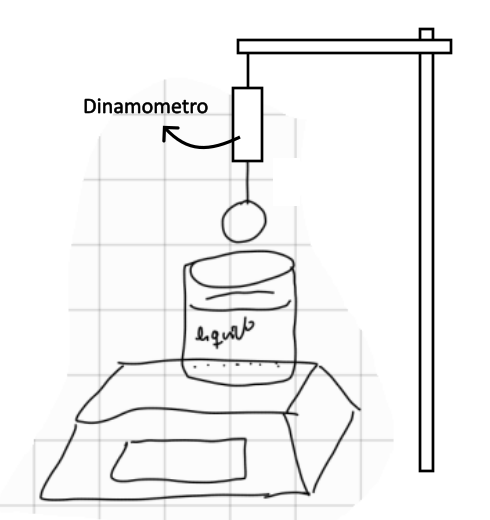
\includegraphics[width = 5cm]{img/img3.png}
        \caption{\label{arr} Arreglo experimental}
    \end{figure}     

    



 
   

    \subsection{Análisis de los datos}

    Resulta necesario tener todo en las mismas unidades de primera instancia. El volumen ocupado por la pelota lo podemos conocer con el cambio de altura en el nivel del agua $h$, y el diámetro del vaso $\phi_v$ como:

    \begin{equation}
        V = h \pi (\phi/2)^2
    \end{equation}

    Donde la incertidumbre se propaga como:

    \begin{equation}
        \Delta V = 2r\pi h\Delta r + r^2 \pi \Delta h
    \end{equation}

    De tal forma que el valor obtenido al final, ya en metros cuadrados, es: $V = (7.67 \pm 0.05) \times 10^{-5}$m$^3$.
    Respecto a los pesos, digamos que $w_{b0}$ es el de la bola fuera del agua, $w_{b1}$ el que registra el dinamómetro cuando se sumerge (ambos ya en Newtons e indicados en la sección anterior), $w_{a0}$ el del vaso con el agua antes de sumergir la bola, y $w_{a1}$ después de hacerlo. Estos dos últimos datos no los tenemos, pero los podemos obtener con los datos registrados por la bascula, de tal forma que, considerando a $g = (9.78 \pm 0.02)$m/s$^2$ de acuerdo a \cite{inegi} \footnote{En dicho archivo se hacen medidas del valor de $g$ en varias partes de la República Mexicana, donde en promedio para distintas localizaciones y alturas se obtiene dicho valor}, y considerando que el peso esta dado por $W = mg$, tenemos al final los siguientes datos:

    \begin{table}[H] 
    \caption{\label{tab1} Pesos registrados} 
       \begin{center}
       \begin{tabular}{|p{1.5cm}|p{3.2cm}|}
       \hline
        $w_{b0}$ & $(1.525 \pm 0.025)$N \\
       \hline
        $w_{b1}$&$(0.750 \pm 0.025)$N\\
       \hline
        $w_{a0}$ & $(8.493 \pm 0.018)$N \\
        \hline
        $w_{a1}$ & $(9.23 \pm 0.02)$N \\
        \hline
       \end{tabular}
       \end{center}
    \end{table}

    Ahora bien, si la pelota no estuviera sujetada por la cuerda y el dinamómetro al momento de sumergiría, esta se hundiría, y el peso que registraría la bascula seria el equivalente a $w_{b0} + w_{a0}$, que seria: $(10.018 \pm 0.043)$. Notese que si sumamos $w_{b1} + w_{a1}$, esto es igual a: $(9.98 \pm 0.045)$. Notese que las dos sumas anteriores están a menos de una incertidumbre de distancia, de tal forma que en escénica son iguales, lo cual se retoma en la discusión.

    Ahora bien, atendiendo el objetivo central de esta practica, lo que nos interesa saber que se cumpla la eq 2, donde al tener que la pelota se encuentra en equilibro dentro del fluido:
    
    \begin{equation}
        0 = F_b + W + T
    \end{equation}

    Donde solo nos interesan las magnitudes ya que todas las fuerzas se presentan en un solo eje. $F_b$ es la fuerza que ejerce el fluido, $W$ es el peso de la pelota, y $T$ es la tensión. Es fácil ver tomando las consideraciones adecuadas de signos que: $W = -w_{b0}$, y $T = w_{b1}$, la eq 5 queda como:

    \begin{equation}
        F_b = w_{b0} - w_{b1} = (0.775 \pm 0.050)N
    \end{equation}

    Ahora bien, para comprobar el principio de Arquímedes, y la eq 2, bastaría ver que: $\rho g V = F_b$, donde $\rho$ es la densidad del agua, y $V$ el volumen de la pelota.
    Digamos que $W_d$ es el peso del volumen desplazado, que será $W_d = \rho g V$
    El único dato que hace falta es el ultimo, el cual previamente se obtuvo con un valor de: $(998 \pm 2)$kg/m$^3$. Bajo las consideraciones anteriores, y además tomando en cuenta que: $\Delta W_d = V \rho \Delta g + Vg \Delta \rho + g \rho \Delta V$:

    \begin{equation}
        W_d = (0.759 \pm 0.008)N
    \end{equation}

    \end{multicols}


    \vspace{0.7cm}    

    \hline

    \section{Resolución}

    \hline

    \begin{multicols}{2}
    
        \subsection{Discusión}

        Respecto a lo que sucede al sumergir la pelota, y el porque cambia el valor medido de la báscula, es debido a que parte del peso total de la pelota no es contrarrestado por el fluido, si no que parte de él es contrarrestado por la cuerda. Recordemos que al final lo que mide una bascula es la fuerza normal que requiere para sostener lo que tiene arriba suyo, y en este caso, dado que la tensión de la cuerda aguanta el peso. Esto lo podemos afirmar al ver que los valores de $w_{b0} + w_{a0}$ y de $w_{b1} + w_{a1}$ se aproximan, y se contienen en sus incertidumbres. 

        Respecto a comparar que la fuerza boyante se asemejara al peso del volumen desplazado, es fácil ver que los valores de $F_b$ y $W_d$ se aproximan y se contienen por lo menos en dos veces el valor de sus incertidumbres.


 
        \subsection{Conclusión: }

        Durante este experimento se logró cumplir el objetivo establecido previamente, que requería que se demostrara experimentalmente el Principio de Arquímedes. Como se ve en el análisis de resultados y la discusión, los resultados experimentales concuerdan con lo esperado teóricamente.

        \subsection{Bibliografía}
    
        \begin{thebibliography}{9}
        \bibitem{hamb} Hewitt, P. G. (2016). Física Conceptual. 12 Ed. Pearson.
        \bibitem{inegi} Instituto Nacional de Estadística y Geografía, INEGI (2021). Estaciones de gravedad absoluta en México. Recuperado de \url{https://www.inegi.org.mx/contenidos/productos/prod_serv/contenidos/espanol/bvinegi/productos/nueva_estruc/702825198435.pdf} el 1 de Octubre del 2024.

        \end{thebibliography}


    \end{multicols}
            
    \hline

    \vspace{1cm}

  
	
\end{document}